\documentclass[aspectratio=169,10pt]{beamer}
\usepackage{common/pdmtheme}
\graphicspath{{figures/}}
\title[nRF9160 node]{Nordic nRF9160}
\subtitle{Cellular node --- no gateway, and the longest battery life in the lineup}
\author{Predictive Maintenance Platform}
\date{13 October 2026}
\begin{document}

\begin{frame}[plain]
  \vspace{5mm}
  {\LARGE\bfseries Nordic nRF9160}\\[2mm]
  {\large\color{pdmink2} Cellular node: no gateway, 9.4 years}\par
  \vspace{5mm}\noindent{\color{pdmrule}\rule{\linewidth}{0.4pt}}\par
  \vspace{3mm}
  \begin{columns}[T]
    \begin{column}{0.46\textwidth}
      \scriptsize
      \kv{MCU}{nRF9160 SiP, M33 @ 64 MHz}\\[1mm]
      \kv{Radio}{LTE-M + GNSS, integrated modem}\\[1mm]
      \kv{Sensor}{IIS3DWB on SPI3}\\[1mm]
      \kv{RAM}{\textbf{256 kB} --- the binding constraint}\\[1mm]
      \kv{Pipeline}{101 kB after two optimisations}\\[1mm]
      \kv{Battery life}{\textbf{9.4 y} hourly, D-cell LiSOCl$_2$}
    \end{column}
    \begin{column}{0.46\textwidth}
      \scriptsize\color{pdmink2}
      \textbf{Never flashed.} The LTE energy figures are the least certain
      numbers in this repository --- Nordic app-note arithmetic, and real
      networks vary by operator, band and how the operator configures PSM. A
      2$\times$ error would move 9.4 years to between 5 and 19.
      \\[2mm]
      It is also the only kit that reports a \emph{measured} sample rate.
    \end{column}
  \end{columns}
  \srcnote{Branch \texttt{hw/nrf9160-cellular}.}
\end{frame}

% ------------------------------------------------------------- the result ----
\begin{frame}{The most expensive radio has the longest battery life}
  \centering
  \scriptsize
  \begin{tabular}{@{}lrrrr@{}}
    \toprule
    & \textbf{Radio per TX} & \textbf{Cell} & \textbf{Self-disch.} & \textbf{Life, hourly} \\
    \midrule
    STWIN.box, BLE   & 0.29 mA$\cdot$s & 480 mAh LiPo & 20 $\mu$A & 1.6 y \\
    \textbf{nRF9160, LTE-M} & \textbf{95 mA$\cdot$s} & D LiSOCl$_2$ & \textbf{4 $\mu$A} & \textbf{9.4 y} \\
    ESP32-S3, Wi-Fi  & 240 mA$\cdot$s & 18650 Li-ion & 72 $\mu$A & 1.7 y \\
    \bottomrule
  \end{tabular}
  \\[3mm]
  \begin{columns}[T]
    \begin{column}{0.47\textwidth}
      \scriptsize
      330$\times$ the radio energy of BLE and 5.8$\times$ the life. The
      mechanism is not the radio:
      \\[1mm]
      {\tiny\ttfamily
      LTE-M pulses 200-250 mA\\
      ~-> within a LiSOCl2 D-cell's capability\\
      ~~~-> self-discharge 0.08 \%/month = 4 uA\\
      ~~~~~-> circuit (40 uA) dominates\\
      ~~~~~~~-> the design actually matters -> 9.4 y
      \\[1mm]
      Wi-Fi bursts 350 mA\\
      ~-> outside LiSOCl2's pulse capability\\
      ~~~-> forces Li-ion, 2.5 \%/month = 72 uA\\
      ~~~~~-> cell dominates above hourly\\
      ~~~~~~~-> saturates at 2.7 y, firmware irrelevant
      }
    \end{column}
    \begin{column}{0.49\textwidth}
      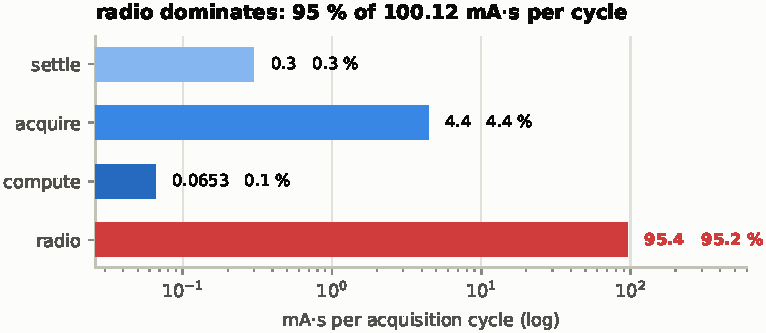
\includegraphics[width=\linewidth]{kit_nrf9160_energy.pdf}
    \end{column}
  \end{columns}
  \takeaway{On a low-duty sensor, battery life is usually a chemistry decision
    dressed up as a firmware problem. Three of our five battery kits have a cell
    whose self-discharge exceeds the circuit's draw.}
\end{frame}

% ------------------------------------------------------------------- RAM -----
\begin{frame}{256 kB forced two optimisations every kit should adopt}
  \centering
  \scriptsize
  \begin{tabular}{@{}lrr@{}}
    \toprule
    & \textbf{Naive} & \textbf{This kit} \\
    \midrule
    Raw int16 FIFO staging          & 49\,152 & \textcolor{pdmgood}{\textbf{0}} \\
    Window + twiddle + bit-reversal & 46\,096 & \textcolor{pdmgood}{\textbf{0}} (flash) \\
    Acquisition \texttt{float[8192]}& 32\,768 & 32\,768 \\
    Envelope \texttt{float[8192]}   & 32\,768 & 32\,768 \\
    FFT in place                    & 16\,384 & 16\,384 \\
    Magnitude + spectrum            & 16\,392 & 16\,392 \\
    Chunk scratch                   & ---     & 3\,072 \\
    \midrule
    \textbf{Total}                  & \textbf{168 kB} & \textbf{101 kB} \\
    \bottomrule
  \end{tabular}
  \\[3mm]
  \begin{columns}[T]
    \begin{column}{0.48\textwidth}
      \scriptsize
      \textbf{1. No raw staging buffer.} Each 512-sample FIFO chunk is converted
      to float \emph{as it arrives}, through a 3 kB scratch. Saves 48 kB and
      costs nothing --- the conversion was going to happen anyway. The other
      kits stage the raw block because they can afford to, which is a weak
      reason.
    \end{column}
    \begin{column}{0.48\textwidth}
      \scriptsize
      \textbf{2. Tables in flash.} 46 kB of a 1 MB part buys 46 kB of a 256 kB
      part, and removes $\sim$40 ms of boot transcendentals.
      \\[1mm]
      Second-order effect: that boot cost is one-off on a kit that retains SRAM
      and \emph{per-cycle} on one that does not --- so the optimisation is worth
      most on the ESP32-S3, even though the nRF9160 forced it.
      \\[1mm]
      \texttt{make -C cdsp test-flash-tables}: 0 of 43 features differ, worst
      2.4e-6.
    \end{column}
  \end{columns}
\end{frame}

% ------------------------------------------------------------------ PSM ------
\begin{frame}{Two radio decisions worth more than any DSP optimisation}
  \begin{columns}[T]
    \begin{column}{0.48\textwidth}
      \small\textbf{PSM, not System OFF}
      \\[1.5mm]
      \scriptsize
      \begin{tabular}{@{}lr@{}}
        \toprule
        RRC connection (registered) & $\sim$95 mA$\cdot$s \\
        Full LTE attach             & $\sim$1000 mA$\cdot$s \\
        \bottomrule
      \end{tabular}
      \\[2mm]
      System OFF reaches $\sim$2 $\mu$A against PSM's $\sim$3 $\mu$A --- and
      drops the registration, so every wake pays an attach. Saving 3.6
      mA$\cdot$s per hour to spend 905 is a bad trade \textbf{by a factor of
      250}.
      \\[1.5mm]
      The PSM parameters are \emph{requests}. An operator that grants a 1-hour
      TAU instead of 10.5 turns a 9-year node into a 2-year one --- which is why
      verifying the granted values with \texttt{AT+CEREG?} is on the checklist
      and is not a formality.
    \end{column}
    \begin{column}{0.48\textwidth}
      \small\textbf{NB-IoT fallback disabled}
      \\[1.5mm]
      \scriptsize
      Better coverage, $\sim$10$\times$ worse latency. A modem that falls back
      automatically changes the energy budget by an order of magnitude
      \emph{without telling anyone}, and the symptom is a fleet where some nodes
      mysteriously have a quarter of the expected life.
      \\[1.5mm]
      If a site needs NB-IoT that is a per-device deployment decision in the
      asset registry, not something the modem decides at 3 a.m.
      \\[2.5mm]
      \small\textbf{Snapshots at most daily}
      \\[1mm]
      \scriptsize
      A 51 kB waveform is $\sim$540 s of airtime and $\sim$2\,600 mA$\cdot$s ---
      \textbf{27 acquisitions' worth of energy for one waveform.}
    \end{column}
  \end{columns}
\end{frame}

% ------------------------------------------------------------- rate ----------
\begin{frame}{The only kit that measures its own sample rate}
  \begin{columns}[T]
    \begin{column}{0.5\textwidth}
      \small
      \texttt{k\_uptime\_get()} runs from the 32.768 kHz LFCLK --- a
      $\pm$20 ppm crystal. Timing a 307 ms acquisition to 1 ms resolution gives
      \texttt{samples / elapsed} to \textbf{0.33 \%}, against the IIS3DWB
      oscillator's $\pm$3 \% specification.
      \\[2mm]
      \scriptsize
      The STWIN.box \emph{cannot} do this: nothing there times the acquisition
      against a crystal, so its fix needs a reference tone through the self-test
      actuator. The ESP32-S3 could and does not yet.
    \end{column}
    \begin{column}{0.46\textwidth}
      \scriptsize
      \textbf{Why 3 \% matters, concretely.}
      \\[1mm]
      A 3 \% error computes a 106.3 Hz BPFO line as if it were at 103.1 Hz. The
      matcher's tolerance is $\pm$2 \% with a 1.5-bin floor, so the fundamental
      still matches.
      \\[1mm]
      By the \textbf{fifth harmonic} the error is 16 Hz against a $\pm$10.6 Hz
      window. The harmonic falls outside, and \texttt{n\_matched} drops from 5 to
      3 or 4.
      \\[1mm]
      \texttt{n\_matched} is one of the 63 features the detector was
      \emph{trained} on. So a kit with a 3 \% rate error produces systematically
      different features from one with 0.3 \% --- on the same machine.
    \end{column}
  \end{columns}
  \takeaway{Implemented here, identified-and-not-done on the ESP32-S3, and
    needing new hardware on the STWIN.box. Three kits, three answers, all written
    down.}
\end{frame}

\end{document}
